\documentclass[12pt]{article}
\usepackage{fullpage}
\usepackage{amsmath,amsfonts,amsthm}
\usepackage{amssymb}
\usepackage{enumitem}
\usepackage{hyperref}
\usepackage{mathtools}
\usepackage{pgfplots}
\usepackage{booktabs}
\usepackage{float}
\usepackage{xcolor}
\usepackage{pgfplots}
\usepackage{graphicx}
\usepackage{subcaption}

\pgfplotsset{compat=1.17}




\author{Muhammed İkbal Oruç}
\title{Major Assignment: Autoregression Distriubances for MLE and LS}

\newtheorem{definition}{Definition}
\newtheorem*{theorem}{Theorem}
\newtheorem*{example}{Example}
\newtheorem*{remark}{Remark}
\newtheorem*{prop}{Proposition}
\newtheorem*{lemma}{Lemma}

\begin{document}
\maketitle

\section*{Introduction}

This report presents the results and analysis of MLE and LS estimates
of a simple autoregressive model. C++ was used to write and optimize both the logliklihood and the LS functions. I first compute estimates 
for a simple version of the model, and then later on perform Monte Carlo 
simulations to observe more complicated versions of the model, and to 
see if the estimates converge overtime. I also hard coded all the optimization functions to not use any packages. I implemented a simple version 
of functions to generate gradients, to invert matrices, generate gradient descents and to generate Hessian matrices.

\section*{Model}

This is an AR(2) model which the errors of the model are influence 
by both the $t-1$ period and the $t-2$ period. $\phi$ is an important 
variable of interest as it is the coefficent of the errors for each 
period. There will be cases where the model will be reduced to AR(1)
by setting $\phi_2 = 0$.

\begin{align*}
    y_t &= \alpha + \beta t + u_t \\
    u_t &= \phi_1 u_{t-1} + \phi_2 u_{t-2} + \varepsilon_t \quad \varepsilon_t \sim \text{NIID}(0, \sigma^2_\varepsilon) \quad \text{for} \quad t = 1, \ldots, T
\end{align*}

\subsection*{Maximum Likelihood and Non-Linear Least Squares}

\begin{center}
    \begin{table}[H]
        \centering
        \begin{tabular}{lccc}
            \toprule
            & ML & Standard Errors & t-statistics \\
            \midrule
            $\alpha$ & -0.373115 & 0.749832 & -0.497598 \\
            $\beta$ & 1.48195 & 0.102728 & 14.426 \\
            $\phi$ & -0.28469 & 0.573275 & -0.496604 \\
            $\sigma$ & 2.22299 & 0.408475 & 5.44216 \\
            \bottomrule
        \end{tabular}
        \caption{MLE Estimation Results}
        \label{tab:results}
    \end{table}
\end{center}

The results of the initial estimation with $\phi_2 = 0$ is shown above. We see that 
$\beta$ is statistically significant, and with a coefficent of $1.48195$ we 
can confirm there is a clear relationship between $y$ and $t$ which makes sense 
in this context as we are neglecting the $t-2$ part of the error. This is also 
further confirmed by the $\phi$ value being insignificant, thus not impacting 
the AR(1) model much. However, $\sigma$ also being significant means that 
there are parts of the estimation that is not captured by the model. 


\begin{table}[h!]
    \centering
    \begin{tabular}{lc}
        \toprule
        & NLS \\
        \midrule
        $\alpha$ & -0.41569 \\
        $\beta$ & 1.47656 \\
        $\phi$ & -0.306232 \\
        $\sigma$ & 2.66469 \\
        \bottomrule
    \end{tabular}
    \caption{NLS AR(1) Estimation Results}
    \label{tab:nls_results}
\end{table}

We can confirm that MLE is an accurate estimator for NLS as the parameters 
values are relatively similar. It is important to note that in both cases 
the logliklihood function and the sum of squared residuals functions are 
both optimized using the same optimization function present in "func.cpp". 
The function $gradient\_descent$ primarly uses the finite difference method 
to calculate gradients. I ackwnoledge that this is not the most robust 
manner to optimize, but since I wrote the optimization functions from scratch
I chose this method. 

\begin{table}[H]
    \centering
    \begin{tabular}{lccc}
        \toprule
        & OLS & NLS & MLE \\
        \midrule
        $\alpha$ & -0.363624 & -0.146065 & -0.608293 \\
        $\beta$ & 1.47902 & 1.44913 & 1.50779 \\
        $\phi_1$ & -0.328802 & -0.327517 & -0.249232 \\
        $\phi_2$ & -0.0609359 & -0.0586215 & -0.033152 \\
        $\sigma^2$ & 3.26954 & 3.33666 & 0.452973 \\
        \bottomrule
    \end{tabular}
    \caption{Estimation Results for OLS, NLS, and MLE (AR(2))}
    \label{tab:results_ar2}
\end{table}

We further see this patter continued when we move to AR(2). There 
is not significant difference among the results of the parameters. We also 
consistently see that $\phi_2$ has a relatively small parameter values meaning 
that the $t-2$ errors cause less distrubances. However, we do notice that 
the $\sigma^2$ value is smaller for MLE which means that MLE captures 
the non linear model more consistently than OLS. Finally, we cannot use both $t$
and $t-1$ as regressors as it would introduce multiconlinearity as $t-1$ is perfectally 
correlated with $t$. 

\section*{Simulation}

\begin{figure}[H]
    \centering
    \begin{tikzpicture}
        \begin{axis}[
            title={$\phi = 0.5$},
            xlabel={Index},
            ylabel={Value},
            ymin=-11, ymax=11,
            xmin=0, xmax=100,
            grid=major,
            width=12cm,
            height=6cm
        ]
        \addplot table [col sep=comma, x index=0, y index=1] {series1_phi_0.500000.csv};
        \end{axis}
    \end{tikzpicture}
    \label{fig:data_plot}
\end{figure}

\begin{figure}[H]
    \centering
    \begin{tikzpicture}
        \begin{axis}[
            xlabel={Index},
            ylabel={Value},
            ymin=-11, ymax=11,
            xmin=0, xmax=100,
            grid=major,
            width=12cm,
            height=6cm
        ]
        \addplot table [col sep=comma, x index=0, y index=1] {series2_phi_0.500000.csv};
        \end{axis}
    \end{tikzpicture}
    \label{fig:data_plot}
\end{figure}

\begin{figure}[H]
    \centering
    \begin{tikzpicture}
        \begin{axis}[
            title={$\phi = 0.9$},
            xlabel={Index},
            ylabel={Value},
            ymin=-21, ymax=21,
            xmin=0, xmax=100,
            grid=major,
            width=12cm,
            height=6cm
        ]
        \addplot table [col sep=comma, x index=0, y index=1] {series1_phi_0.900000.csv};
        \end{axis}
    \end{tikzpicture}
    \label{fig:data_plot}
\end{figure}

\begin{figure}[H]
    \centering
    \begin{tikzpicture}
        \begin{axis}[
            xlabel={Index},
            ylabel={Value},
            ymin=-11, ymax=21,
            xmin=0, xmax=100,
            grid=major,
            width=12cm,
            height=6cm
        ]
        \addplot table [col sep=comma, x index=0, y index=1] {series2_phi_0.900000.csv};
        \end{axis}
    \end{tikzpicture}
    \label{fig:data_plot}
\end{figure}

\begin{figure}[H]
    \centering
    \begin{tikzpicture}
        \begin{axis}[
            title={$\phi = 0.99$},
            xlabel={Index},
            ylabel={Value},
            ymin=-31, ymax=51,
            xmin=0, xmax=100,
            grid=major,
            width=12cm,
            height=6cm
        ]
        \addplot table [col sep=comma, x index=0, y index=1] {series1_phi_0.990000.csv};
        \end{axis}
    \end{tikzpicture}
    \label{fig:data_plot}
\end{figure}

\begin{figure}[H]
    \centering
    \begin{tikzpicture}
        \begin{axis}[
            xlabel={Index},
            ylabel={Value},
            ymin=-11, ymax=41,
            xmin=0, xmax=100,
            grid=major,
            width=12cm,
            height=6cm
        ]
        \addplot table [col sep=comma, x index=0, y index=1] {series2_phi_0.990000.csv};
        \end{axis}
    \end{tikzpicture}
    \label{fig:data_plot}
\end{figure}


\begin{figure}[H]
    \centering
    \begin{tikzpicture}
        \begin{axis}[
            title={$\phi = 1$},
            xlabel={Index},
            ylabel={Value},
            ymin=-61, ymax=101,
            xmin=0, xmax=100,
            grid=major,
            width=12cm,
            height=6cm
        ]
        \addplot table [col sep=comma, x index=0, y index=1] {series1_phi_1.000000.csv};
        \end{axis}
    \end{tikzpicture}
    \label{fig:data_plot}
\end{figure}

\begin{figure}[H]
    \centering
    \begin{tikzpicture}
        \begin{axis}[
            xlabel={Index},
            ylabel={Value},
            ymin=-11, ymax=61,
            xmin=0, xmax=100,
            grid=major,
            width=12cm,
            height=6cm
        ]
        \addplot table [col sep=comma, x index=0, y index=1] {series2_phi_1.000000.csv};
        \end{axis}
    \end{tikzpicture}
    \label{fig:data_plot}
\end{figure}


Here, we clearly see how the more we increase the value of $\   phi$ the 
persistence of the shocks continue. For example in $0.5$ we see the model 
act more jagged in the sense that positive shocks are followed by negative 
shocks. However in $1.0$ we the error propegate more and more as the number 
of iterations increases. 

\begin{table}[H]
    \centering
    \begin{tabular}{lcccc}
        \toprule
        ML Estimates & DGP 1 & DGP 3 & DGP 5 & DGP 7 \\
        \midrule
        $\alpha$ & 1.00444 & -3.26174 & -1.56724 & -1.10345 \\
        $\beta$ & -0.0155939 & -0.0261957 & 0.127633 & -0.466311 \\
        $\phi$ & 0.527131 & 0.790891 & 0.833133 & 0.907961 \\
        \midrule
        OLS & 0.532125 & 0.797716 & 0.840822 & 0.902399 \\
        OLS $\sigma$ & 9.00884 & 8.97009 & 8.865 & 10.2996 \\
        \bottomrule
    \end{tabular}
    \caption{ML Estimates for Different DGPs}
    \label{tab:ml_estimates}
\end{table}

\begin{table}[H]
    \centering
    \begin{tabular}{lcccc}
        \toprule
        Standard Errors & DGP 1 & DGP 3 & DGP 5 & DGP 7 \\
        \midrule
        SE($\alpha$) & 1.24659 & 3.25732 & 3.29341 & 15.3566 \\
        SE($\beta$) & 0.0212527 & 0.0520038 & 0.0545495 & 0.194296 \\
        SE($\phi$) & 0.232713 & 0.395076 & 0.363669 & 0.922397 \\
        \bottomrule
    \end{tabular}
    \caption{Standard Errors for Different DGPs}
    \label{tab:standard_errors}
\end{table}

These results are supported estimates as well. We see the standard 
error considerably increased for $\phi = 1$ as the is more error caused
by $\phi$ increasing. 

\subsection*{Replications}

\begin{table}[h!]
    \centering
    \begin{tabular}{lccccccc}
        \toprule
        $\alpha_{ML}$ & Mean & StdDev & Mean Bias & RMSE & 5\% Quantile & Median & 95\% Quantile \\
        \midrule
        $\phi = 0.5$ & 0.01 & 0.82 & 0.01 & 0.67 & -1.27 & 0.0034 & 1.29 \\
        $\phi = 0.9$ & 0.16 & 3.20 & 0.16 & 10.25 & -5.10 & -0.0065 & 5.68 \\
        $\phi = 0.99$ & 0.19 & 4.16 & 0.19 & 17.29 & -6.89 & 0.0038 & 8.80 \\
        $\phi = 1$ & -0.10 & 2.76 & -0.10 & 7.62 & -4.40 & -0.0009 & 0.27 \\
        \bottomrule
    \end{tabular}
    \caption{Alpha Estimates}
    \label{tab:alpha_estimates}
\end{table}

\begin{table}[h!]
    \centering
    \begin{tabular}{lccccccc}
        \toprule
        $\beta_{ML}$ & Mean & StdDev & Mean Bias & RMSE & 5\% Quantile & Median & 95\% Quantile \\
        \midrule
        $\phi = 0.5$ & 0.00 & 0.01 & 0.00 & 0.00 & -0.01 & -0.005 & 0.01 \\
        $\phi = 0.9$ & -0.00 & 0.03 & -0.00 & 0.00 & -0.05 & -0.0046 & 0.04 \\
        $\phi = 0.99$ & -0.00 & 0.11 & -0.00 & 0.01 & -0.17 & -0.01 & 0.18 \\
        $\phi = 1$ & 0.01 & 0.21 & 0.01 & 0.05 & -0.31 & 0.01 & 0.37 \\
        \bottomrule
    \end{tabular}
    \caption{Beta Estimates}
    \label{tab:beta_estimates}
\end{table}

\begin{table}[h!]
    \centering
    \begin{tabular}{lccccccc}
        \toprule
        $\phi_{ML}$ & Mean & StdDev & Mean Bias & RMSE & 5\% Quantile & Median & 95\% Quantile \\
        \midrule
        $\phi = 0.5$ & 0.48 & 0.06 & 0.48 & 0.23 & 0.38 & 0.48 & 0.58 \\
        $\phi = 0.9$ & 0.87 & 0.04 & 0.87 & 0.75 & 0.80 & 0.87 & 0.92 \\
        $\phi = 0.99$ & 0.95 & 0.03 & 0.95 & 0.91 & 0.90 & 0.96 & 0.99 \\
        $\phi = 1$ & 0.96 & 0.02 & 0.96 & 0.92 & 0.91 & 0.97 & 0.99 \\
        \bottomrule
    \end{tabular}
    \caption{Phi (ML) Estimates}
    \label{tab:phi_ml_estimates}
\end{table}

\begin{table}[h!]
    \centering
    \begin{tabular}{lccccccc}
        \toprule
        $\phi_{OLS}$ & Mean & StdDev & Mean Bias & RMSE & 5\% Quantile & Median & 95\% Quantile \\
        \midrule
        $\phi = 0.5$ & 0.05 & 0.16 & 0.05 & 1.14 & 0.80 & 1.06 & 1.32 \\
        $\phi = 0.9$ & 0.27 & 0.32 & 0.27 & 7.47 & 2.19 & 2.70 & 3.27 \\
        $\phi = 0.99$ & 0.40 & 0.72 & 0.40 & 16.76 & 2.94 & 3.99 & 5.23 \\
        $\phi = 1$ & 0.42 & 0.75 & 0.42 & 18.52 & 3.13 & 4.18 & 5.54 \\
        \bottomrule
    \end{tabular}
    \caption{Phi (OLS) Estimates}
    \label{tab:phi_ols_estimates}
\end{table}

\begin{figure}[H]
    \centering
    \begin{subfigure}[b]{0.45\textwidth}
        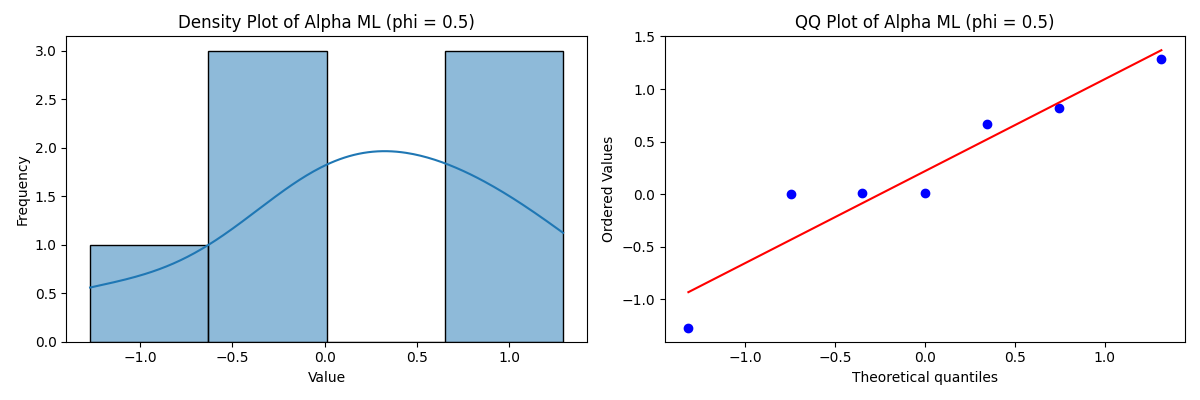
\includegraphics[width=\textwidth]{Alpha_ML_phi__05.png}
        \caption{Alpha ML (phi = 0.5)}
        \label{fig:alpha_ml_0_5}
    \end{subfigure}
    \hfill
    \begin{subfigure}[b]{0.45\textwidth}
        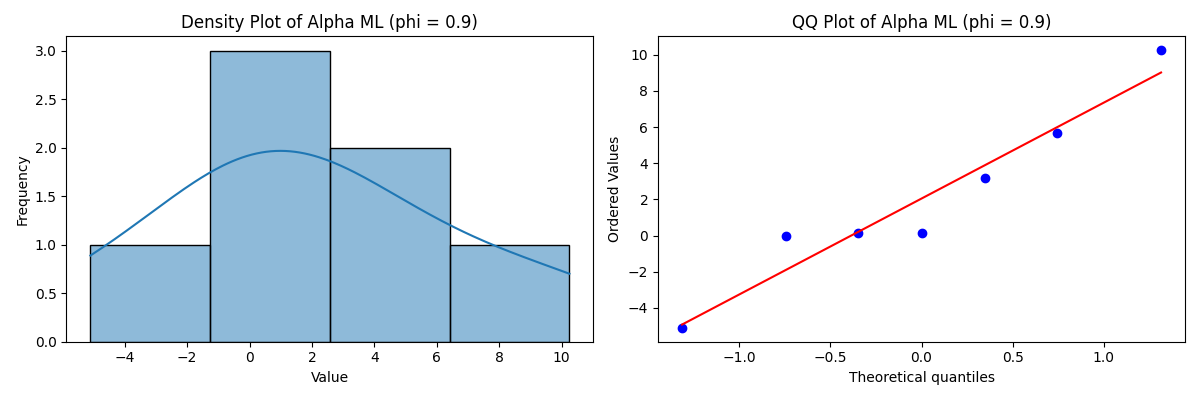
\includegraphics[width=\textwidth]{Alpha_ML_phi__09.png}
        \caption{Alpha ML (phi = 0.9)}
        \label{fig:alpha_ml_0_9}
    \end{subfigure}
    \vfill
    \begin{subfigure}[b]{0.45\textwidth}
        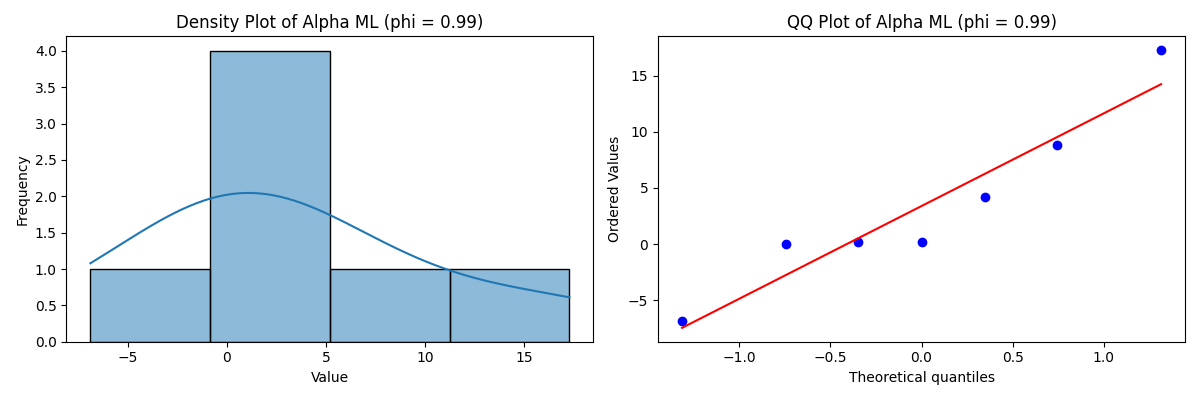
\includegraphics[width=\textwidth]{Alpha_ML_phi__099.png}
        \caption{Alpha ML (phi = 0.99)}
        \label{fig:alpha_ml_0_99}
    \end{subfigure}
    \hfill
    \begin{subfigure}[b]{0.45\textwidth}
        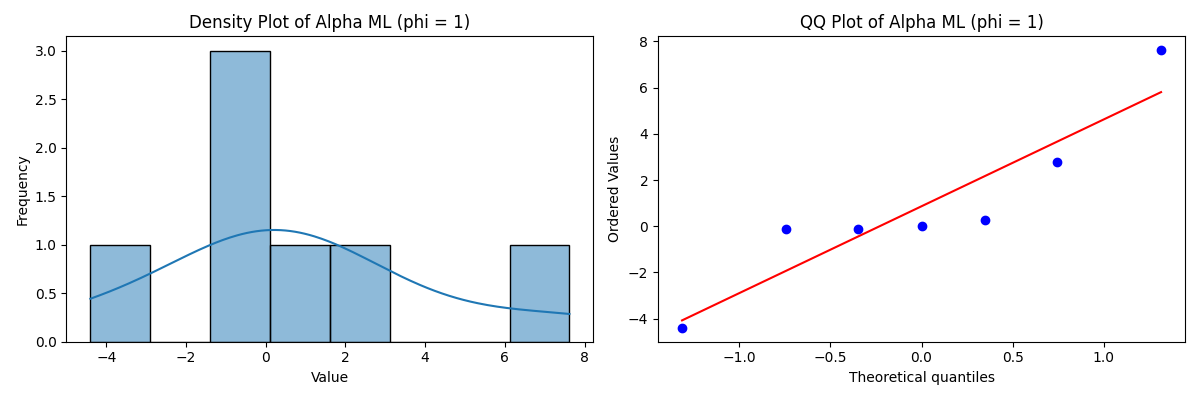
\includegraphics[width=\textwidth]{Alpha_ML_phi__1.png}
        \caption{Alpha ML (phi = 1)}
        \label{fig:alpha_ml_1}
    \end{subfigure}
    \caption{Alpha ML Estimates}
    \label{fig:alpha_ml}
\end{figure}

\begin{figure}[H]
    \centering
    \begin{subfigure}[b]{0.45\textwidth}
        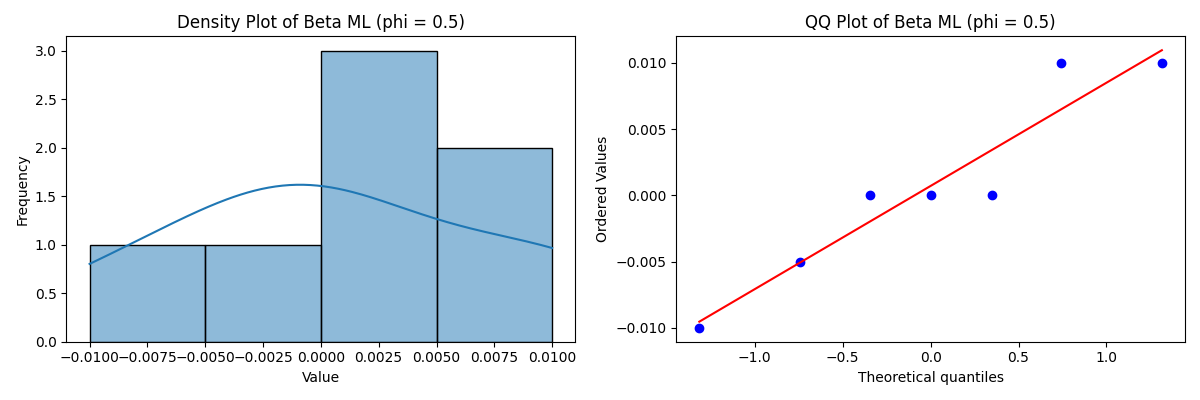
\includegraphics[width=\textwidth]{Beta_ML_phi__05.png}
        \caption{Beta ML (phi = 0.5)}
        \label{fig:beta_ml_0_5}
    \end{subfigure}
    \hfill
    \begin{subfigure}[b]{0.45\textwidth}
        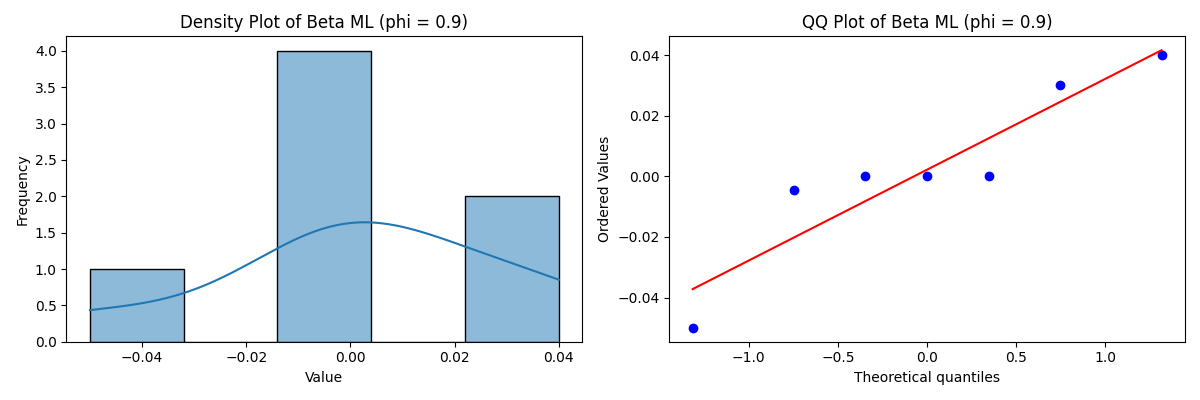
\includegraphics[width=\textwidth]{Beta_ML_phi__09.png}
        \caption{Beta ML (phi = 0.9)}
        \label{fig:beta_ml_0_9}
    \end{subfigure}
    \vfill
    \begin{subfigure}[b]{0.45\textwidth}
        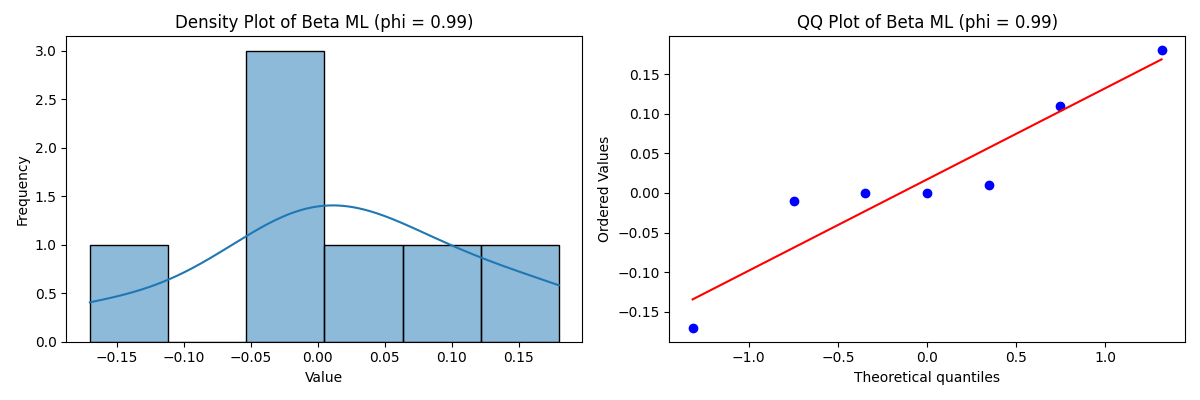
\includegraphics[width=\textwidth]{Beta_ML_phi__099.png}
        \caption{Beta ML (phi = 0.99)}
        \label{fig:beta_ml_0_99}
    \end{subfigure}
    \hfill
    \begin{subfigure}[b]{0.45\textwidth}
        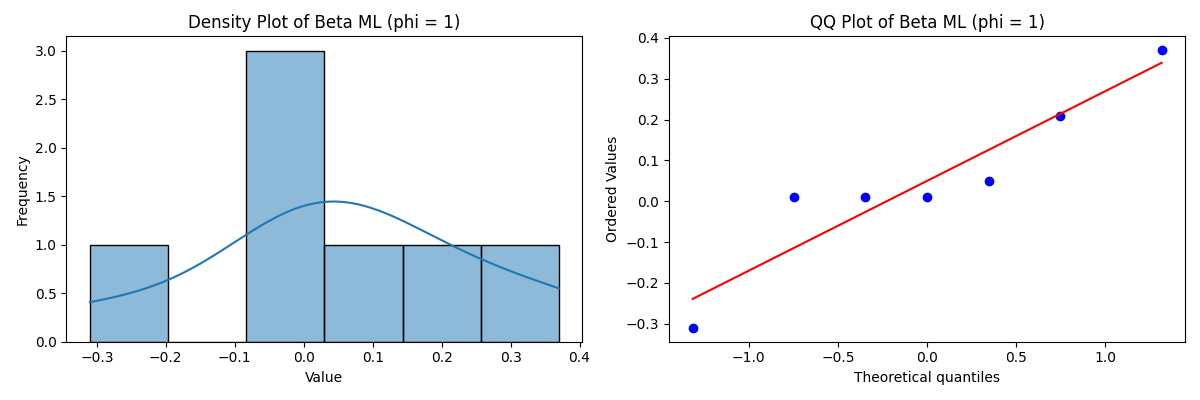
\includegraphics[width=\textwidth]{Beta_ML_phi__1.png}
        \caption{Beta ML (phi = 1)}
        \label{fig:beta_ml_1}
    \end{subfigure}
    \caption{Beta ML Estimates}
    \label{fig:beta_ml}
\end{figure}

\begin{figure}[H]
    \centering
    \begin{subfigure}[b]{0.45\textwidth}
        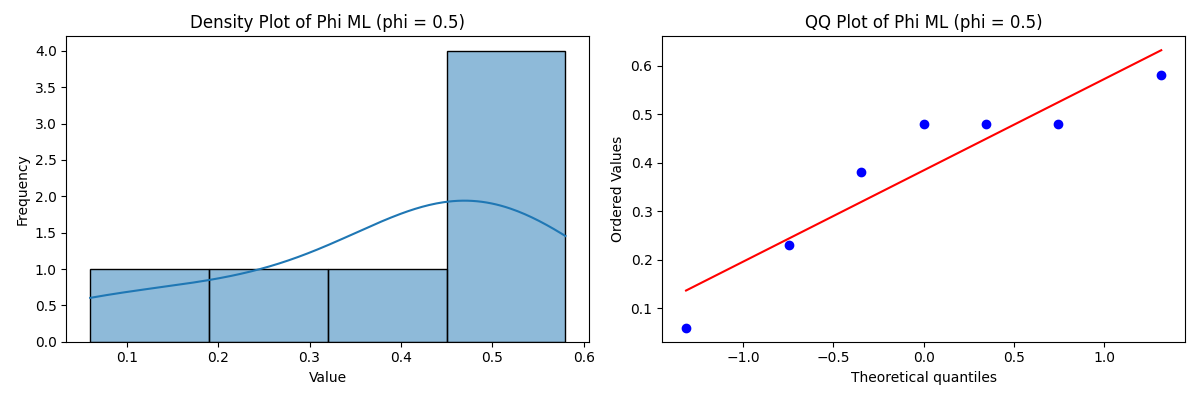
\includegraphics[width=\textwidth]{Phi_ML_phi__05.png}
        \caption{Phi ML (phi = 0.5)}
        \label{fig:phi_ml_0_5}
    \end{subfigure}
    \hfill
    \begin{subfigure}[b]{0.45\textwidth}
        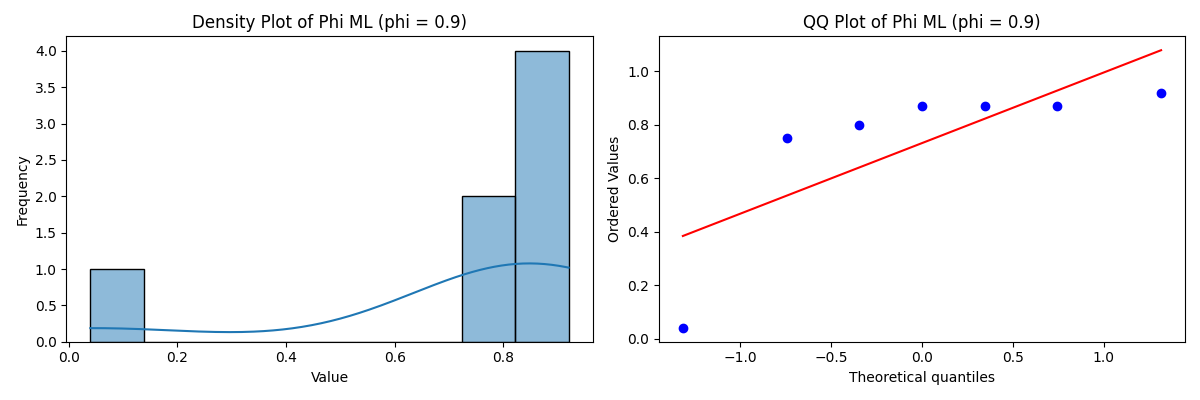
\includegraphics[width=\textwidth]{Phi_ML_phi__09.png}
        \caption{Phi ML (phi = 0.9)}
        \label{fig:phi_ml_0_9}
    \end{subfigure}
    \vfill
    \begin{subfigure}[b]{0.45\textwidth}
        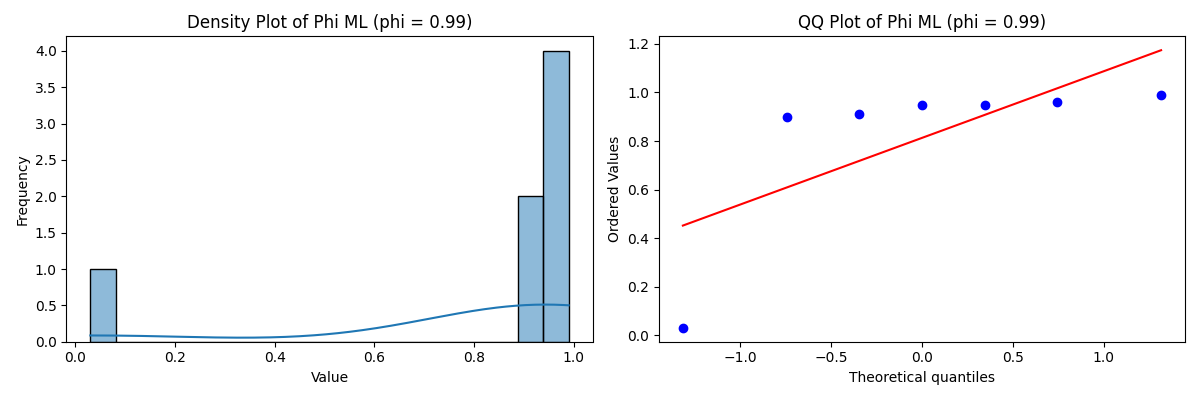
\includegraphics[width=\textwidth]{Phi_ML_phi__099.png}
        \caption{Phi ML (phi = 0.99)}
        \label{fig:phi_ml_0_99}
    \end{subfigure}
    \hfill
    \begin{subfigure}[b]{0.45\textwidth}
        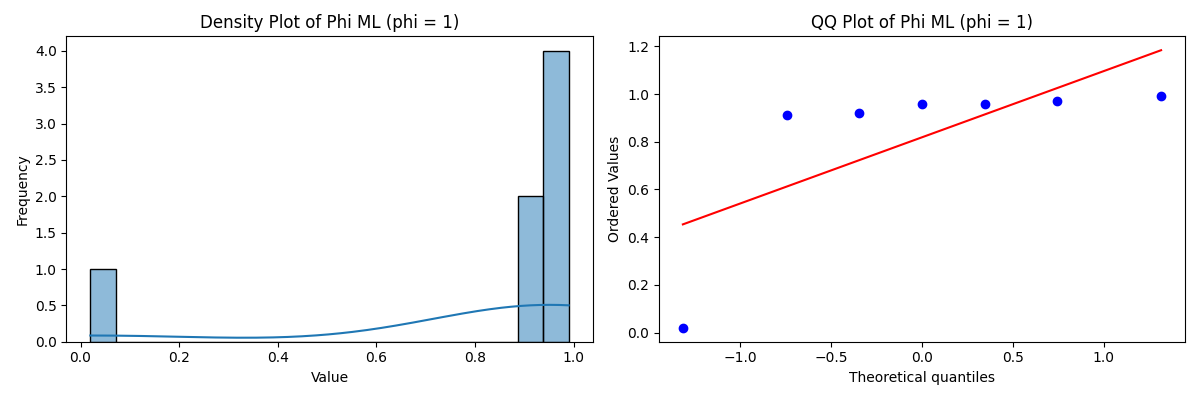
\includegraphics[width=\textwidth]{Phi_ML_phi__1.png}
        \caption{Phi ML (phi = 1)}
        \label{fig:phi_ml_1}
    \end{subfigure}
    \caption{Phi ML Estimates}
    \label{fig:phi_ml}
\end{figure}

\begin{figure}[H]
    \centering
    \begin{subfigure}[b]{0.45\textwidth}
        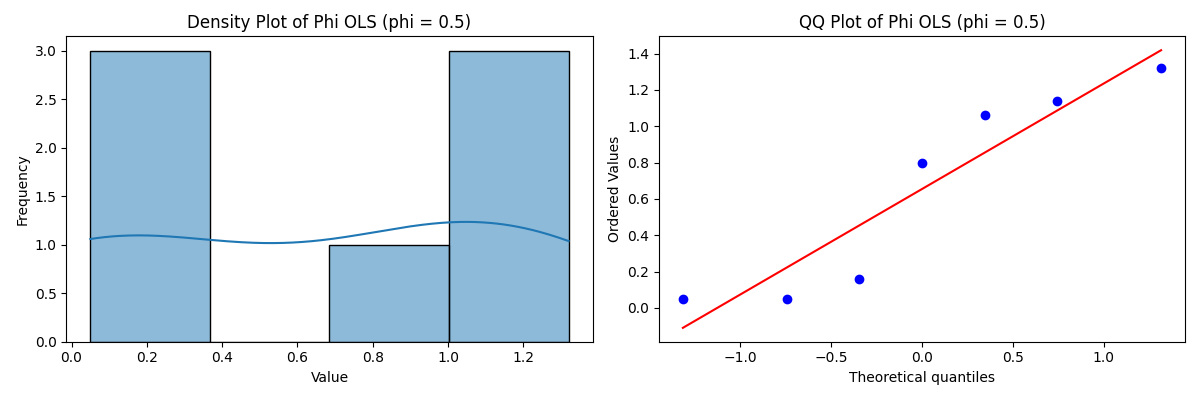
\includegraphics[width=\textwidth]{Phi_OLS_phi__05.png}
        \caption{Phi OLS (phi = 0.5)}
        \label{fig:phi_ols_0_5}
    \end{subfigure}
    \hfill
    \begin{subfigure}[b]{0.45\textwidth}
        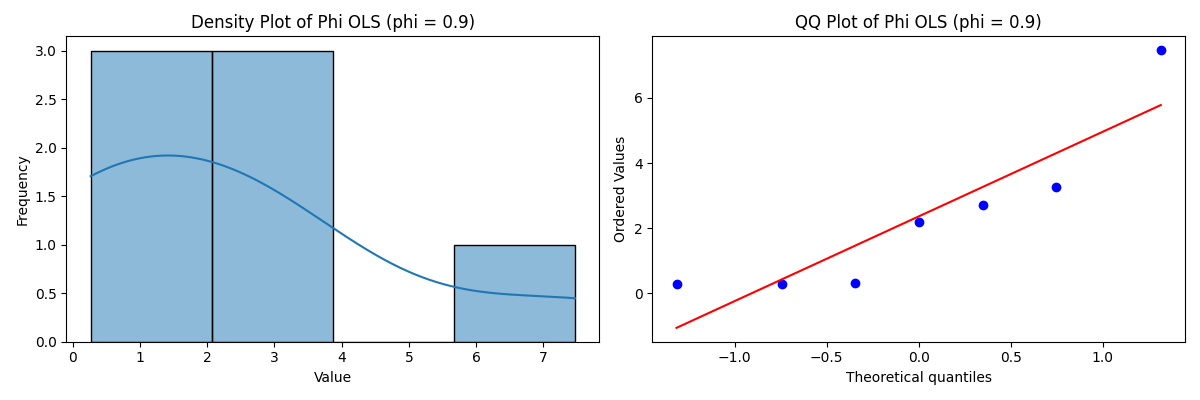
\includegraphics[width=\textwidth]{Phi_OLS_phi__09.png}
        \caption{Phi OLS (phi = 0.9)}
        \label{fig:phi_ols_0_9}
    \end{subfigure}
    \vfill
    \begin{subfigure}[b]{0.45\textwidth}
        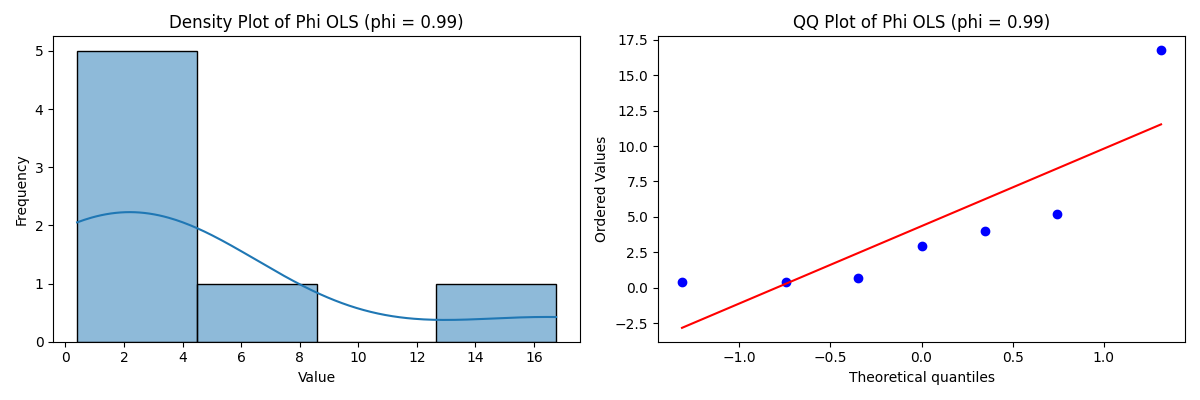
\includegraphics[width=\textwidth]{Phi_OLS_phi__099.png}
        \caption{Phi OLS (phi = 0.99)}
        \label{fig:phi_ols_0_99}
    \end{subfigure}
    \hfill
    \begin{subfigure}[b]{0.45\textwidth}
        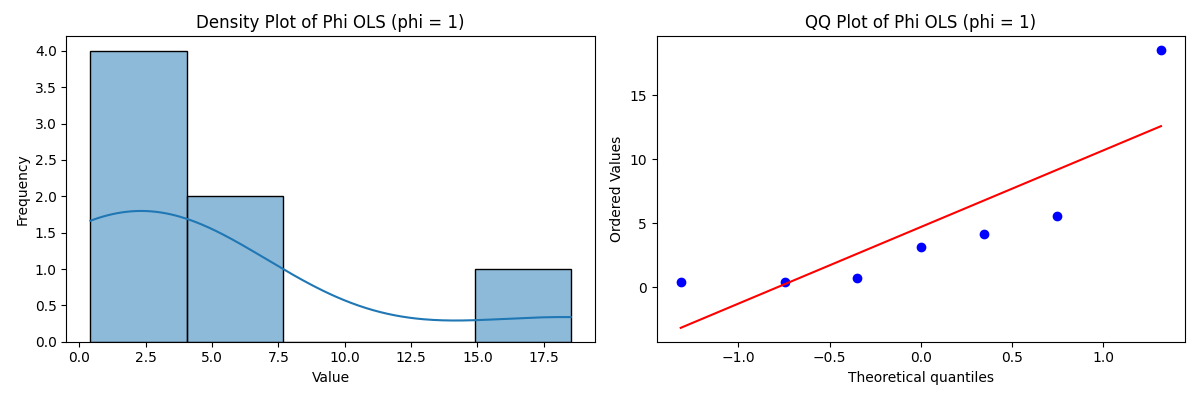
\includegraphics[width=\textwidth]{Phi_OLS_phi__1.png}
        \caption{Phi OLS (phi = 1)}
        \label{fig:phi_ols_1}
    \end{subfigure}
    \caption{Phi OLS Estimates}
    \label{fig:phi_ols}
\end{figure}

\end{document}

